\documentclass[12pt]{exam}
\newcommand{\hwnumber}{4}
\newcommand{\hwname}{DosLingos}
\newcommand{\duedate}{\formatdate{14}{02}{\YEAR} by \progDueTime}

\usepackage{../misc/latex/edition}  % Course semester
\usepackage{../misc/latex/c0}       % Listings style for c0
\usepackage{amsmath}
\usepackage{enumerate}
\usepackage[normalem]{ulem}
\usepackage{verbatim}
\usepackage[left=1in, right=1in, top=1in, bottom=1in]{geometry}
\usepackage{graphicx}
\usepackage{hyperref}
\usepackage{tikz}     \usetikzlibrary{shapes}
\usepackage{fancybox}
\usepackage[all]{xy}
\usepackage{wrapfig}
\usepackage{fancyvrb}
\usepackage{datetime}
\usepackage{etoolbox}
\usepackage{calc}
\usepackage[nomessages]{fp}
\usepackage{import}  % Like input and include, but respects subdirectories

\newcommand{\defaultQuestionLocation}{questions}
\newcommand{\inputQuestion}[2][\defaultQuestionLocation/]{%
  \subimport{#1}{#2}
}
% Subdirectories of \defaultQuestionLocation containing code and pictures
\newcommand{\code}{code}
\newcommand{\img}{img}


%%% ic: frontmatter macros
\newcommand{\specialInstructions}{}
\newcommand{\HWNUMBER}
{\ifdefempty{\hwnumber}{__}{%
  \ifnumless{\hwnumber}{10}{0\hwnumber}{\hwnumber}}}
\newcommand{\hwtype}{Written Homework}

%%% ic: 'exam' tweaks
\renewcommand{\half}{.5} % Half points

\newcommand{\Question}[2][]
 {\ifstrempty{#1}
    {\question{\bf #2}}
    {\question[#1]{\bf #2}}
  \immediate\write\rubricfile{}%
  \immediate\write\rubricfile{Question \thequestiontitle:}%
  \immediate\write\rubricfile{==========}
 }

%%% ic: Support for editable PDF
% counter name (some viewers misbehave if always the same)
\newcounter{editable}
\newcommand{\nextField}{\addtocounter{editable}{1}q\arabic{editable}}
\newcommand{\NextField}
 {\makebox[0pt][r]{\scalebox{0.1}{\color{White}\nextField}}}

% Color of edit area
\newcommand{\editAreaColor}{red}
% Single line answer:   \editableLine[extra parameters (optional)]{line width}
\newcommand{\editableLine}[2][]
{\textcolor{\editAreaColor}{%
 \underline{\hspace*{-0.25em}%
 \raisebox{-0.5ex}{%
 \TextField[width=#2, borderwidth=0, #1]{\NextField}}}}%
}
% Single line answer for code:  \editableLine[extra parameters (optional)]{line width}
\newcommand{\editableCodeLine}[2][]
{\textcolor{\editAreaColor}{%
 \underline{%
 \TextField[width=#2, height=1.5ex, borderwidth=0, #1]{\NextField}}}}
% Multiline answer:  \editableLine[extra parameters (optional)]{box height}
\newcommand{\editableBox}[2][]
{\leavevmode\hspace*{-0.1em}%
\TextField[height=#2, width=\linewidth,
           multiline=true, borderwidth=0.1, bordercolor=\editAreaColor,
           #1]{\NextField}}

%%%%% Same answer format as exams
\renewcommand{\rmdefault}{ppl}
\renewcommand{\sfdefault}{phv}
\newcommand{\answerColor}{Blue}

\ifprintanswers
\newcommand{\answer}[2]{\makebox[#1][c]{\color{\answerColor}#2}}
\else
\newcommand{\answer}[2]{\makebox[#1][c]{}\makebox[0pt]{\phantom{|}}}
\fi
\newcommand{\uanswer}[2]{\underline{\answer{#1}{#2}}}


%%% Write rubric snippet.  Usage:
% \RUBRIC
% any multi-line text (including \, #, %, whatever)
% ENDRUBRIC
%% (ENDRUBRIC should be on a line by itself)
\makeatletter
\def\RUBRIC
 {%
  \begingroup
  \let\do\@makeother\dospecials
  \endlinechar=`\^^J
  \@tofile%
 }
\def\ENDRUBRIC{ENDRUBRIC}
\def\@tofile#1^^J{%
  \def\@test{#1}%
  \ifx\@test\ENDRUBRIC
    \immediate\write\rubricfile{}  % End with an empty line
    \expandafter\@firstoftwo
  \else
    \expandafter\@secondoftwo
  \fi
  {\endgroup}%
  {\toks@{#1}%
   \begingroup\endlinechar=\m@ne
   \everyeof{\noexpand}%
   \xdef\@temp{\scantokens\expandafter{\the\toks@}}%
   \endgroup
   \immediate\write\rubricfile{\@temp}%
   \@tofile}%
}
\makeatother

%% Displays tags for an exercise in 'answer' mode
\newcommand{\TAGS}[1]
{\ifprintanswers%
  \rule{0em}{0ex}%
  \marginpar{\footnotesize%
    \fcolorbox{black}{Gray!25}{%
      \parbox[t]{2cm}{\raggedright\textbf{TAGS:}\\#1}}}%
  \ignorespaces%
 \fi}%


%% Page layout
\pagestyle{headandfoot}

\headrule
\header{\textbf{\courseNumber{} \hwtype{} \hwnumber}}
       {}
       {\textbf{Page \thepage\ of \numpages}}
\footrule
\footer{}{}{\COPYRIGHT}

\renewcommand{\partlabel}{\textbf{\thequestion.\thepartno}}
%\renewcommand{\partlabel}{\textbf{Task \thepartno}}
\renewcommand{\subpartlabel}{\textbf{\thesubpart.}}
\renewcommand{\thepartno}{\arabic{partno}}
\renewcommand{\thesubpart}{\alph{subpart}}
\pointpoints{pt}{pts}
\pointformat{\raisebox{0ex}[\height][0pt]{\fcolorbox{black}{yellow}{\themarginpoints}}}
\bonuspointformat{\raisebox{0ex}[\height][0pt]{\fcolorbox{black}{red}{\themarginpoints}}}
\marginpointname{\points}
\pointsinmargin
%\boxedpoints

\setlength\answerlinelength{2in}
\setlength\answerskip{0.3in}

\newcommand{\mkWrittenTitle}[1]{#1}
\newcommand{\mkDueDate}[1]{#1}
\newcommand{\mkEvalSummary}[1]{#1}
\newcommand{\mkGradetable}[1]{#1}



% This fixes an issue with the exam package version 2.6 and after,
% where 'framed' has been renamed to 'examframed' to avoid a conflict.
\ifcsmacro{examframed}{%
\newenvironment{framed}
{\begin{examframed}}
{\end{examframed}}
}{}


\newif\ifAnalysisVersionA % S18 S15
\newif\ifAnalysisVersionB % S19 S17 F16 S16
%\AnalysisVersionAtrue
\AnalysisVersionBtrue

\begin{document}
\hwTitle

\noindent
This week we will do some relatively small exercises centered around
searching and sorting arrays of integers and strings. We compared
characters and strings for equality during the puzzle hunt portion of
our first programming assignment; Appendix~\ref{sec:strings} of this
writeup talks a little big more about string comparison, which is
necessary when we think about sorted arrays of strings.

\bigskip
\noindent
The code handout for this assignment is on \autolab{} and at
\begin{center}
\whereisthetgz{doslingos-handout.tgz}
\end{center}

The file \lstinline'README.txt' in the code handout goes over the contents
of the handout and explains how to hand the assignment in.  There is
a FIVE (5) PENALTY-FREE HANDIN LIMIT.
Every additional handin will incur a small (5\%) penalty (even if
using a late day).
 {\bf Be aware that only Task 3 will be graded
  by Autolab when you hand in your work. You should examine Autolab's
  output to make sure the other tasks compile. \emph{If you
    don't check Autolab's outputs and there are compilation errors,
    you may end up receiving no credit for the assignment.}}

The other tasks will be autograded or graded by hand after the
assignment deadline. You will need to use the test cases you write for
task 3, contracts, and deliberate programming to ensure correctness of
the other tasks.

\newpage
\section{DosLingos (Counting Common Words)}
\label{sect:common}

\paragraph{The story:} %
You're working for a Natural Language Processing (NLP) startup company called
DosLingos.\footnote{Any resemblance between this scenario and Dr.\@ Luis von
  Ahn's company DuoLingo (\url{http://www.duolingo.com}) are \emph{purely}
  coincidental.}  Already, your company has managed to convince thousands of
users to translate material from English to Spanish for free. In a recent
experiment, you had users translate newswire text and you've managed to train
your users to recognize words in an English newspaper.  Now you're considering
having these same users translate Shakespeare, and you're not sure how many
words your Spanish-speaking users will be able to recognize.

%\clearpage
\paragraph{Your job:}
In this exercise, you will write a function for analyzing the number
of tokens from a text corpus (like the complete works of Shakespeare)
that appear (or not) in a user's vocabulary. The user's expected
vocabulary will be represented by a sorted array of strings
\lstinline"vocab" that has length \lstinline"v", and we will maintain another
integer array, \lstinline"freq", where \lstinline"freq[i]" represents the number
of times we have seen \lstinline"vocab[i]" in the text corpus so far (where $i \in
[0,v)$).

\begin{center}
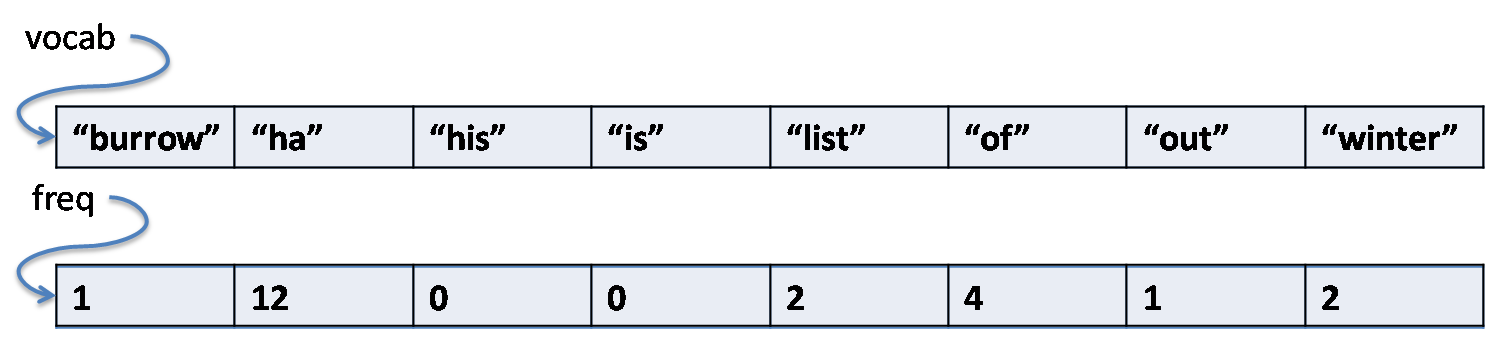
\includegraphics[width=0.7\textwidth]{img/array-before.png}
\end{center}

\noindent
This is an important pattern, and one that we will see repeatedly
throughout the semester in 15-122: the (sorted) vocabulary words
stored in \lstinline'vocab' are \emph{keys} and the frequency counts stored
in \lstinline'freq' are \emph{values}.

The function \lstinline'count_vocab' that we will write updates the values
--- the frequency counts --- based on the text corpus we are analyzing.
As an example, consider a text made up not from Shakespeare but
from this tweet by local weatherman Scott Harbaugh:

\begin{center}
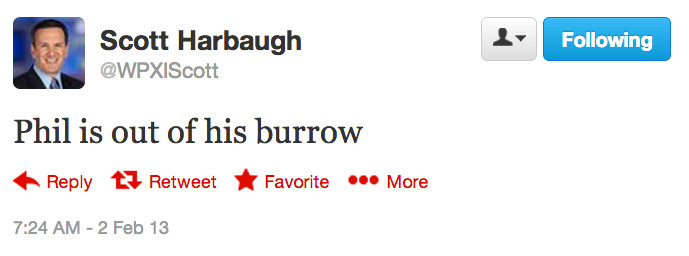
\includegraphics[width=0.6\textwidth]{img/wpxiscott.png}
\end{center}

\noindent
We would expect
\lstinline'count_vocab(vocab,freq,8,"texts/scott_tweet.txt",b)' to return 1 (because
only one word, ``Phil,'' is not in our example vocabulary), leave the
contents of \lstinline'vocab' unchanged, and update the frequency counts in
\lstinline'freq' as follows:

\begin{center}
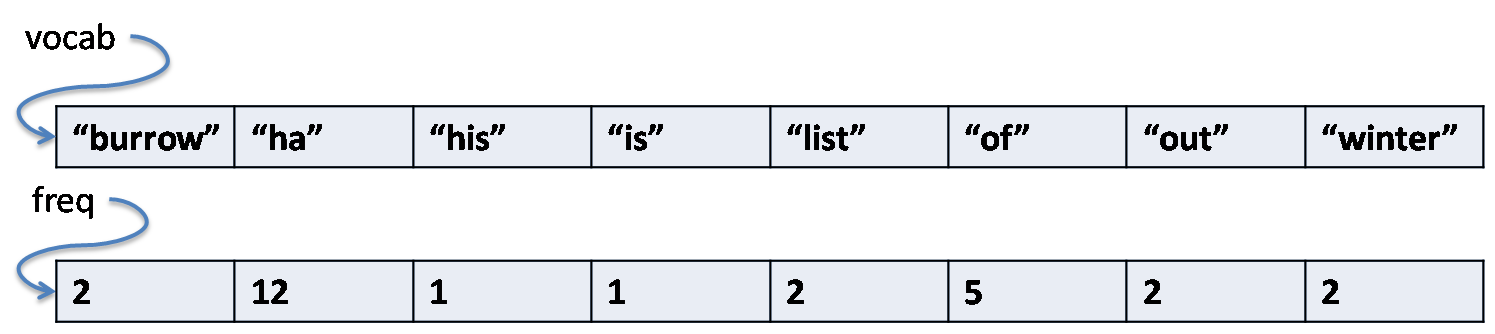
\includegraphics[width=0.7\textwidth]{img/array-after.png}
\end{center}

\paragraph{Your data:} DosLingos has given you 4 data files for your project
in the \lstinline'texts/' directory:
\begin{itemize}
\item \lstinline"news_vocab_sorted.txt" - A sorted list of vocabulary words from news text that DosLingos users are familiar with.
\item \lstinline"scott_tweet.txt" - Scott Harbaugh's tweet above.
\item \lstinline"sonnets.txt" - A small test file: 122 of Shakespeare's sonnets.
\item \lstinline"shakespeare.txt" - A larger test file: the complete works
  of Shakespeare.
\end{itemize}
You can write more data files of your own!

\paragraph{Your tools:}

DosLingos already has a C0 library for reading text files,
converting all letters to lowercase, and separating out words,
provided to you as \lstinline"lib/readfile.c0", which defines a type
\lstinline'bundle_t' and implements the following functions:

\begin{quote}
\begin{lstlisting}[numbers=none]
// first call read_words to read in the content of the file
bundle_t read_words(string filename)
\end{lstlisting}
\end{quote}
You need not understand anything about the type \lstinline"bundle_t"
other than that you can
extract its underlying \lstinline"string" array and the length of that array:
\begin{quote}
\begin{lstlisting}[numbers=none]
// to determine the length of the array in the string_bundle, use:
int string_bundle_length(bundle_t sb)

// access the array inside of the string_bundle using:
string[] string_bundle_array(bundle_t sb)
//@ensures \length(\result) == string_bundle_length(sb);
\end{lstlisting}
\end{quote}

\noindent
Here's an example of these functions being used on Scott Harbaugh's
tweet:

\begin{quote}
\begin{lstlisting}[language={[coin]C}]
% coin -d lib/readfile.c0
--> bundle_t B = read_words("texts/scott_tweet.txt");
B is 0x7047F0 (struct string_bundle_header*)
--> string_bundle_length(B);
6 (int)
--> string[] tweet = string_bundle_array(B);
tweet is 0x704B60 (string[] with 6 elements)
--> tweet[0];
"phil" (string)
--> tweet[5];
"burrow" (string)
\end{lstlisting}
\end{quote}

Being connoisseurs of efficient algorithms, DosLingos has also implemented
their own set of string search algorithms in \lstinline"lib/stringsearch.c0", which
you may also find useful for this assignment:
\begin{quote}
\begin{lstlisting}[numbers=none]
// Linear search
int linsearch(string x, string[] A, int n)
//@requires 0 <= n && n <= \length(A);
//@requires is_sorted(A, 0, n);
/*@ensures (-1 == \result && !is_in(x, A, 0, n))
        || ((0 <= \result && \result < n)
            && string_equal(A[\result], x)); @*/


// Binary search
int binsearch(string x, string[] A, int n)
//@requires 0 <= n && n <= \length(A);
//@requires is_sorted(A, 0, n);
/*@ensures (-1 == \result && !is_in(x, A, 0, n))
        || ((0 <= \result && \result < n)
            && string_equal(A[\result], x)); @*/
\end{lstlisting}
\end{quote}



The code for this exercise should be put in a file
\lstinline'doslingos.c0'. You must include annotations for the
precondition(s), postcondition(s) and loop invariant(s) for each
function. You may include additional annotations for assertions as
necessary.
% Note that you are
% given some specification functions (e.g. \texttt{is\_sorted}) in your
% downloaded code.
You may include any auxiliary functions you need in the same file, but
you should not include a \lstinline"main()" function.  You can include
functions from the \lstinline'lib/readfile.c0' and \lstinline'lib/stringsearch.c0'
libraries in your code: the compilation instructions given in
\lstinline'README.txt' include these libraries.

%% These two tasks should be placed in a file \lstinline'doslingos.c0'
%% Your tests should be put in a file \lstinline'doslingos-test.c0' that has a
%% \lstinline'main()' function. The autograder will test your tests and
%% give feedback, but these
%% tests will not contribute to your grade.


\begin{task}[4]
\TAGS{array, loop-invariant, safety, sorting}
Add to \lstinline'doslingos.c0' a definition of the function
\lstinline'count_vocab':
\begin{quote}
\begin{lstlisting}[numbers=none]
int count_vocab(string[] vocab, int[] freq, int v,
                string corpus,
                bool fast)
//@requires v == \length(vocab) && v == \length(freq);
//@requires is_sorted(vocab, 0, v);
//@requires all_distinct(vocab, v);
\end{lstlisting}
\end{quote}
The function should return the number of occurrences of words in the
file \lstinline"corpus" that do not appear in the array
\lstinline"vocab", and should update the frequency counts in
\lstinline'freq' with the number of times each word in the vocabulary
appears.  If a word appears multiple times in the \lstinline"corpus",
you should count each occurrence separately, so a file containing ``ha
ha ha LOL LOL'' would cause the frequency count for ``ha'' to be
incremented by 3 and would cause 2 to be returned, assuming LOL was
not in the vocabulary. (It should not be an error if this addition
causes overflow. The easiest thing to do is just increment the
frequency counts without regard to overflow, and you should do that.)

Note that a precondition of \lstinline"count_vocab" is that the
\lstinline"vocab" must be sorted, a fact you should exploit.  Your function
should use the linear search algorithm when \lstinline"fast" is set to
\lstinline'false' and it should use the binary search algorithm when \lstinline"fast"
is \lstinline'true'.  {\em You can implement this choice with a simple
  if statement that decides which function to call --- duplicating a
  lot of code is unnecessary and unhelpful.}

The precondition \lstinline'all_distinct(vocab, v)' enforces that there are
no duplicate words. You DO NOT have to write this function or include
this part of the precondition; we promise not to test your code on any
sorted vocabularies with duplicate words. However, you may write and
include an \lstinline'all_distinct' precondition if you want to. If you
write it, include it in the same file \lstinline'doslingos.c0'.

\end{task}


%\clearpage
\section{Sorting by Frequency}

To really utilize our frequency counts, it is useful to be able to
take our vocabulary list and frequency counts and re-arrange both
arrays so that the frequency counts are sorted.
\begin{center}
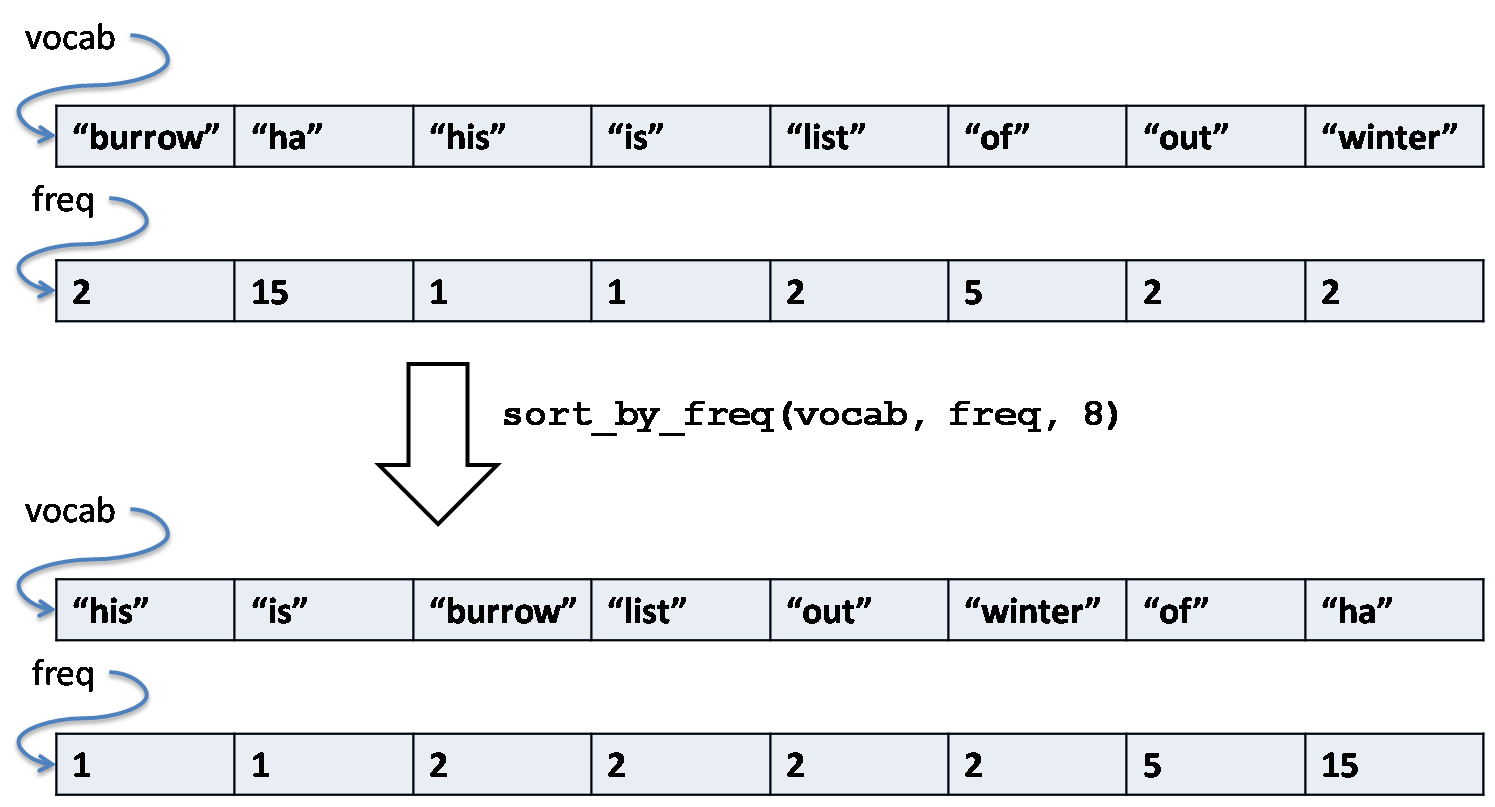
\includegraphics[width=0.7\textwidth]{img/array-resort.png}
\end{center}
You'll want to adapt one of the sorting functions we discussed in
lecture for this task (in other words, it's okay to start with the
lecture code and modify it). You'll need to modify the lecture code so
that it sorts the two arrays \emph{together}. In the example above,
when we move 15 from index 1 to index 7 in \lstinline'freq', we also have
to move ``ha'' from index 1 to index 7 in \lstinline'vocab'.
In principle, it's not too hard to adapt
an integer array sorting algorithm to an algorithm that sorts two
arrays: whenever you swap two elements in the array you're sorting
(\lstinline'freq'), make sure the same swap is performed on the other array
(\lstinline'vocab').

For full credit on this task, you will need to give a sorting
algorithm that is \textbf{fast} and \textbf{stable}. By fast, we mean
that it will be $O(n \log n)$ on the inputs we will give it. By
stable, we mean that the relative positions of equivalent elements
(words with the same frequencies) in the inputs are preserved in the
output. The quicksort algorithm we discussed in class would meet the
\textbf{fast} criteria: while it is $O(n^2)$ in the worst case, this
behavior won't be triggered by our frequency counts in our text
corpus.  However, the quicksort algorithm from lecture \textbf{isn't
  stable}. If you straightforwardly adapt quicksort, the words
``burrow'', ``list'', ``out'', and ``winter'' are likely to end up in
a different order, resulting in an output that doesn't match the
example above. (Selection sort is neither fast nor stable.)

The easiest way to make a fast, stable sort is probably to modify
mergesort, which we talked about briefly in class; code for mergesort
is published alongside the lecture notes on
divide-and-conquer sorting.  You're also welcome to try and implement
a stable \lstinline'partition' function, which will make quicksort stable.

\begin{task}[7]
\TAGS{array, complexity, correctness, divide-and-conquer, safety, sorting}
Add to \lstinline'doslingos.c0' a definition of the function
\lstinline'sort_by_freq':
\begin{quote}
\begin{lstlisting}[numbers=none]
void sort_by_freq(string[] vocab, int[] freq, int v)
//@requires v == \length(vocab) && v == \length(freq);
//@ensures is_sorted_int(freq, 0, v);
\end{lstlisting}
\end{quote}
You can adapt any code from lecture, but cite the source in a
comment. Remember that the \lstinline'arrayutil.c0' you're using for this
assignment is for dealing with string arrays, not integer arrays, so
most lecture code won't compile at first. It's okay to remove
contracts that depend on the lecture version of \lstinline'arrayutil.c0'
from your sort, but at least leave enough contracts to reason about the
safety of your code.
\end{task}

\section{Unit testing}

The functions you wrote in the first two tasks could fail in many
ways. On certain inputs, they might fail internal assertions or
postconditions (contract failures), and on other inputs they might
happily return invalid results (contract exploits).

\begin{task}[8]
\TAGS{testing}
Write a file, \lstinline'doslingos-test.c0', that tests your
implementation of your first two tasks.  The autograder will assign
you a grade based on the ability of your unit tests to pass when
given a correct implementation and fail when given various buggy
implementations.  Your tests must still be safe: it should not be
possible for your code to make an array access out-of-bounds when
\lstinline'-d' is turned on.

You do not need to catch all our bugs to get full points, but
catching additional tests will be reflected on the scoreboard.
\end{task}

Because you cannot access all of our buggy implementations except via
the autograder, your grade on this task \emph{will} be given as soon
as you hand in your work.
We'll run tests with contracts (\lstinline'-d') enabled, so the largest
text files should not be used in your unit tests.

You may find it useful to use the functions provided in C0's
\lstinline'parse' library. These functions provide a convenient way
of creating arrays with specific contents.  It's not necessary to use
this library to test your code, but you may find that writing
\begin{quote}
\begin{lstlisting}[numbers=none]
string[] A = parse_tokens("I love 15-122");
\end{lstlisting}
\end{quote}
is more convenient than
writing
\begin{quote}
\begin{lstlisting}[numbers=none]
string[] A = alloc_array(string, 3);
A[0] = "I";
A[1] = "love";
A[2] = "15-122";
\end{lstlisting}
\end{quote}

\subsection*{Testing your tests}

You can test your functions with your own implementation, and with an
awful and badly broken implementation, by running the following
commands:

\begin{quote}
\begin{lstlisting}[language={[coin]C}]
% cc0 -d -w lib/*.c0 doslingos.c0 doslingos-test.c0
% ./a.out
% cc0 -d -w lib/*.c0 doslingos-awful.c0 doslingos-test.c0
% ./a.out
\end{lstlisting}
\end{quote}

Both tests should compile and run, but the last invocation of
\lstinline'./a.out' should trigger a assertion to fail if your tests are
more than minimal. \emph{Even if your test cases fail on the
  awful implementation, they still might not be particularly useful
  test cases.}




%\clearpage
\section{Analyzing the results}
\newcommand{\redacted}
 {\underline{\hspace{1.5em}}\mathtt{REDACTED}\underline{\hspace{1.5em}}}

Once you've carefully tested your \lstinline'doslingos.c0' implementations,
you have a powerful set of tools for analyzing your text corpus. For
the last part of this assignment, you'll run such an analysis.
\emph{It is a violation of the academic integrity policy of this
  course to compare the answers in this section with other students.}

\begin{task}[6]
\TAGS{application, testing}
  Create a file \lstinline"analysis.c0" containing a
  \lstinline'main()' function. We will compile and run this file as
  follows:
\begin{quote}
\begin{lstlisting}[language={[coin]C}]
% cc0 -w -o analysis lib/*.c0 doslingos.c0 analysis.c0
% ./analysis texts/news_vocab_sorted.txt texts/shakespeare.txt
\end{lstlisting}
\end{quote}
Where the first argument if \lstinline'./analysis' is the filename for the
(sorted) dictionary and the second argument is the text corpus.  See
\lstinline'echo.c0' for an example of how to handle command-line
arguments in C0.  Note that, to receive credit, your implementation
shall work for an arbitrary dictionary and an arbitrary corpus ---
possibly much larger than the above example --- passed
as parameters as above.

Your analysis should use the sorted word list to compute and print out
human-readable answers to the following questions:

\ifAnalysisVersionA
\begin{itemize}
\item What are the four most common in-dictionary words in
  the text corpus, and what are their frequencies?
  (Ties, if they occur, can be broken in any way you want.)
\item What in-dictionary words appear exactly 82 times in the text
  corpus?
\item Among the in-dictionary words in the text corpus, what are the
  two smallest frequencies that do not occur? (In the example on the
  top of page 2, the answer would be 3 and 5.)
\item How many times are there fewer words with frequency $f$ than
  there are with frequency $f+1$? (The usual pattern is that, there
  are lots of words that appear 1 time, fewer or the same number of
  words that appear 2 times, and so on. How many times is this pattern
  violated?)
\end{itemize}

Your code only needs to work on reasonable inputs. Specifically, don't
worry about checking that the first argument is a file that is
actually sorted. If you use the tools you developed in this assignment
correctly, you should be able to compute the answers from scratch in a
couple of seconds.
We don't need the output of your analysis to obey a strict format, but
here's the rough format you should follow:
\begin{lstlisting}[language={[coin]C}, mathescape]
The four most common words in the text corpus are:
  1. $\redacted$ (appears $\redacted$ times)
  2. $\redacted$ (appears $\redacted$ times)
  3. $\redacted$ (appears $\redacted$ times)
  4. $\redacted$ (appears $\redacted$ times)

These words appeared 82 times in the text corpus: $\redacted$

There are no words with frequency $\redacted$ or $\redacted$ in the corpus.

In this corpus, there are $\redacted$ times that a frequency f has
strictly fewer words at that frequency than frequency f+1.
\end{lstlisting}
\fi

\ifAnalysisVersionB
\begin{itemize}
\item What are the four most common in-dictionary words in
  the text corpus, and what are their frequencies?
  (Ties, if they occur, can be broken in any way you want.)
\item What in-dictionary words appear exactly 128 times in the text
  corpus?
\item How many in-dictionary words appear exactly once in
  the text corpus? (Don't print them all out, just give
  the number.)
\item How many distinct frequencies (zero counts as a frequency) are
  there for the in-dictionary words in text corpus?  (In the example
  on the top of page 2, the answer would be 5, because 0, 1, 2, 4, and
  12 are the distinct frequencies.)
\end{itemize}

Your code only needs to work on reasonable inputs. Specifically, don't
worry about checking that the first argument is a file that is
actually sorted. If you use the tools you developed in this assignment
correctly, you should be able to compute the answers from scratch in a
couple of seconds.
We don't need the output of your analysis to obey a strict format, but
here's the rough format you should follow:
\begin{lstlisting}[language={[coin]C}, mathescape]
The four most common words in the text corpus are:
  1. $\redacted$ (appears $\redacted$ times)
  2. $\redacted$ (appears $\redacted$ times)
  3. $\redacted$ (appears $\redacted$ times)
  4. $\redacted$ (appears $\redacted$ times)

These words appeared 128 times in the text corpus: $\redacted$

There are $\redacted$ singletons in the corpus.

There are $\redacted$ distinct frequency counts in the corpus.
\end{lstlisting}
\fi
\end{task}

\newpage
\appendix
\section{String Processing Overview}
\label{sec:strings}

In the C0 language, a \lstinline"string" is a sequence of
characters. Unlike languages like C, a string is not the same as an
array of characters. One of the functions in the string library
(which you include in your code by \lstinline+#use <string>+) is
\lstinline'string_compare':
\begin{quote}
\begin{lstlisting}[numbers=none]
int string_compare(string a, string b)
//@ensures -1 <= \result && \result <= 1;
\end{lstlisting}
\end{quote}
The \lstinline"string_compare" function performs a \emph{lexicographic}
comparison of two strings, which is essentially the ordering used in a
dictionary, but with character comparisons being based on the characters'
ASCII codes, not just alphabetical. We can convert between the
\lstinline'char' type and the integer ASCII codes with the
\lstinline'char_ord(c)' and \lstinline'char_chr(i)' functions, also available
in the string library.  For this reason, the ordering used here is sometimes
whimsically referred to as ``ASCIIbetical'' order.  A table of all the ASCII
codes is shown in Figure~\ref{fig:asciitable}.  The ASCII value for
\texttt{'0'} is \lstinline'0x30' (48 in decimal), the ASCII code for
\texttt{'A'} is \lstinline'0x41' (65 in decimal) and the ASCII code for
\texttt{'a'} is \lstinline'0x61' (97 in decimal). Note that ASCII codes are
set up so the character \texttt{'A'} is ``less than'' the character
\texttt{'B'} which is less than the character \texttt{'C'} and so on, so the
``ASCIIbetical'' order coincides roughly with ordinary alphabetical order.

\bigskip
\bigskip

\begin{figure}[hb]
\centering
    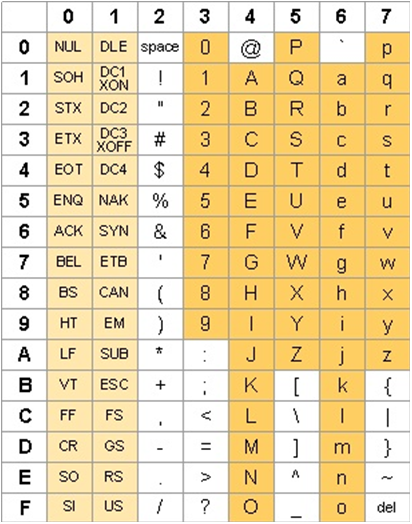
\includegraphics[width=80mm]{img/asciitable.png}
\caption{The ASCII table}
\label{fig:asciitable}
\end{figure}


\end{document}
